\documentclass[conference]{IEEEtran}

\usepackage{cite}
\usepackage{xcolor}
\usepackage{hyperref}
\hypersetup{colorlinks=true,linkcolor=black,citecolor=blue,filecolor=black,urlcolor=blue}
\usepackage{graphicx}
\graphicspath{{figures}}
\usepackage{caption}
\usepackage{subcaption}
\captionsetup[subfigure]{singlelinecheck=false, skip=0pt}
\usepackage{listings}
\renewcommand{\lstlistingname}{Algorithm}
\usepackage[binary-units=true]{siunitx}
\usepackage{csvsimple}
\usepackage{booktabs}
\usepackage{amsmath}
\usepackage{import}

\newcommand{\TG}[1]{\color{blue}\textsc{From Tristan: }#1\color{black}}
\newcommand{\MD}[1]{\color{magenta}\textsc{From Mathieu: }#1\color{black}}
\newcommand{\HL}[1]{\hl{#1}}

\title{An Analysis of Performance Bottlenecks in MRI Pre-Processing}
\author{Mathieu Dugr\'e, Yohan Chatelain, Tristan Glatard}

\begin{document}
\maketitle

\begin{abstract}
	% TODO																
\end{abstract}

\section{Introduction}
% Computational bottleneck
Pre-processing of Magnetic Resonance Imaging (MRI) data is a critical step in neuroimaging. Although established pre-processing pipelines exist, they commonly require expensive computation and produce large output and intermediate data. This has been a major bottleneck to study large subject cohorts in neuroimaging. Moreover, the execution time of pipelines can hinder clinical applications where timely data analysis is needed. For those reasons, the neuroimaging community is constantly seeking ways to improve the performance of MRI pre-processing pipelines.

% HPCs
Researcher broadly adopted High Performance Computing (HPC) to accelerate the MRI processing of large cohorts. HPC systems provide a large number of CPU cores and high-bandwidth memory to process subjects in parallel. However, HPCs might not be available to researchers in developing country. Similarly, cloud computing allows scaling the number of core and memory to process large cohort. However, cloud computing requires expertise to setup and can be costly for large cohort. Moreover, data transfer can be slow and might be impossible due to ethic concerns related to human data. In both cases, the benefits from parallelization are limited by the parallel efficiency of the pipeline and the number of subjects to process. Therefore, it can lead to under-utilization of the available resources.

%  GPUs
\MD{TODO GPUs / Accelerators}

% DL
In recent years, Deep Learning (DL) has shown promising results in MRI pre-preprocessing. For example, tools such as SynthMorph~\cite{Hoffmann2022-hu}, SynthSeg~\cite{Billot2023-vp}, SynthSR~\cite{Iglesias2023-bp}, and SynthStrip~\cite{Hoopes2022-ms} were integrated into FreeSurfer~\cite{Fischl2012-cx} with the effort to provide Deep Learning alternative to traditional algorithms. The main benefit of those tools is the faster runtime they provide. Moreover, A study~\cite{Pepe2023-dm} showed that the results generated by SynthMorph are numerical more stable than those from FreeSurfer. However, training a DL model requires large amount of data and specialized hardware, and is computationally expensive. Additionally, the results from DL models can be challenging to interpret, explaining the slow adoption of DL in MRI pre-processing.

% Alternative solutions
While those techniques can provide significant performance improvements, their additional hardware requirement can be costly and unaccessible to some researchers. Alternatively, improved algorithm designs, compression techniques, or reduced- and mixed-precision techniques could provide substantial performance improvements. However, their implementation can require substantial effort. Therefore, it is critical to understand the performance bottleneck of MRI pre-processing pipelines to improve their performance.

% - No comprehensive study of the performance bottleneck of MRI pre-processing.
The neuroimaging community is well aware that MRI pre-precessing pipelines require long computation time. However, to the best of our knowledge, there is no comprehensive study of the performance bottlenecks in MRI pre-processing. In this paper, we characterize computational cost of several commonly adopted MRI pre-processing pipelines. The results of our analysis serve as a reference for future efforts to optimize MRI pre-processing workflows.

% - Focus on MRI pre-processing.
Magnetic Resonance Imaging (MRI) is a standard tool used by neuroscientists to perform clinical diagnosis and for researchers to develop a better understanding of the brain. Three main MRI techniques exist: structural MRI (sMRI), functional MRI (fMRI), and diffusion MRI (dMRI). While other modalities such as electroencephalogram (EEG), computed tomography (CT), and positron emission tomography (PET) exist, we focus on MRIs for their broad adoption and non-invasive property. Moreover, MRI data analysis is challenging due to computationally expensive pre-processing and large output and intermediate data size.

% - Pipelines
Neuroscientists developed various toolboxes to tackle the challenging task of pre-processing MRI data. We focus on the commonly accepted fMRIPrep~\cite{Esteban2019-bl} workflow as it a comprehensive pre-processing pipeline for both sMRI and fMRI. fMRIPrep combines several pipelines to produce a complete pre-processing workflow. We also study its sub-workflow separately to provide a finer grain analysis of the performance bottleneck.

% - data: OpenNeuro ds004513
We use the OpenNeuro ds004513 v1.0.2 dataset~\cite{ds004513:1.0.2}. We chose this dataset for its wide range of age and equal distribution of biological sex. Using a diverse dataset should help to prevent findings of potential performance bottleneck associated to a specific population.

% - VTune profiler
To profile the pipelines, we use the Intel VTune profiler~\cite{vtune-profiler}. The VTune profiler is a multi-language profiler with low performance overhead and provides information of functions at runtime level. We profile the application using two threading configuration: single-threaded and 32 threads. We aggregate subjects' results for each pipeline to obtain an average performance profile. We compiled each application with debug information to obtain human readable information on function and module names in VTune.

\section{Materials \& Methods}
\subsection{Pipelines}
In this paper, we study the performance bottleneck of fMRIPrep; a commonly used fMRI and sMRI pre-processing workflow. First, we profile the entire workflow to identify the coarse grain performance bottleneck to obtain a coarse view of the workflow's performance. Following, to characterize the performance at a finer grain, we profile the sub-workflows of fMRIPrep: ANTs brainExtraction, ANTs registrationSyN~\cite{Avants2008-ea}, FreeSurfer recon-all~\cite{Dale1999-wu}, FSL FAST~\cite{Zhang2001-hx}, FSL FLIRT~\cite{Jenkinson2002-od,Jenkinson2001-eu,Greve2009-dw}, and FSL MCFLIRT~\cite{Jenkinson2002-od}. We omitted some sub-workflows of fMRIPrep as they were not compatible with our dataset. Moreover, the statistical analysis of the fMRIPrep workflow are not computationally expensive and are not the focus of this paper.

\subsubsection{ANTS registrationSyN}
% Spatial Normalization
% SyN Registration: https://doi.org/10.1016/j.media.2007.06.004
% TODO Mention the option for single and double precision.


\subsubsection{ANTS brainExtraction}
% ANTS brainExtraction
% 1. Truncate image intensity
% 2. N4 bias correction: https://doi.org/10.1109/TMI.2010.2046908
% 3. SyN Registration: : https://doi.org/10.1016/j.media.2007.06.004
% 4. Warp prior to image using affine
% 5. Atropos: https://pubmed.ncbi.nlm.nih.gov/21373993/
% TODO Mention the option for single and double precision.
% TODO OASIS template citation


\subsubsection{FSL FAST}
% DOI: https://doi.org/10.1109/42.906424
% Segmentation


\subsubsection{FreeSurfer recon-all}
% Surface Reconstruction: https://doi.org/10.1006/nimg.1998.0395
% Refer to the fMRIPrep specific 3 stages workflow.


\subsubsection{FSL FLIRT}
% Registration
% FSL FLIRT: https://doi.org/10.1006/nimg.2002.1132, https://doi.org/10.1016/S1361-8415(01)00036-6, https://doi.org/10.1016/j.neuroimage.2009.06.060

\subsubsection{FSL MCFLIRT}
% Head-Motion Correction
% FSL MCFLIRT: https://doi.org/10.1006/nimg.2002.1132

\subsubsection{fMRIPrep}
\MD{TODO import fMRIPrep citation boilerplate from "./fmriprep-citations"}

\subsection{Data}
To ensure the performance profiles of the applications derived from our work are inclusive of different populations, we used data with a wide range of age and equal distribution of sex (biological). Using a diverse dataset should help to prevent findings of potential performance bottleneck associated to a specific population.

We used the the OpenNeuro ds004513 v1.0.2 dataset~\cite{ds004513:1.0.2}. The anatomical, functional, and diffusion data from 20 health individuals was acquired from two different cohorts. The within-subject cohort has nine participants (mean age=43~yrs, std=7~yrs; 4 females) with two session: eyes open and eyes closed. The replication cohort has eleven participants (mean age=27~yrs, std=5~yrs; 6 females) with only the eyes open session. We profiled the application using both cohort on the eyes open session, unless explicitly specified.

\subsection{Profiling}
Profiling MRI pre-processing pipelines present a set of challenges. The neuroimaging community develops pipelines using several programming languages including \textit{C}, \textit{C++}, \textit{Fortran}, \textit{Matlab}, and \textit{Python}, with several pipelines utilizing a combination of multiple languages. Pipelines are generally complex and computationally expensive.

The Intel VTune profiler solves these challenges by offering multi-language support, low performance overhead, and information of functions at runtime level. However, common profiling challenges remain. Profilers require source code to be compiled with Debug Symbols to report useful information about the different functions and modules. Moreover, different input data can substantially vary the analysis due to conditional branching in the application and convergence thresholds. We discuss our approach to these challenges in the next section.
\MD{TODO Cite effect from varying input data on numerical stability and reduced precision. Ask yohan for refereces}
		
First, to obtain human readable information on function and module names in VTune, we re-compiled each pipeline with debug information in a Docker image. For use on HPC systems, we created Apptainer~\cite{Kurtzer2017-bu} images using Docker2Singularity\footnote{\href{https://github.com/singularityhub/docker2singularity}{https://github.com/singularityhub/docker2singularity}} \lstlistingname~\ref{alg:vtune_example} illustrate the profiling of a pipeline by mounting the VTune binary to the Apptainer image at execution.

\begin{minipage}{\linewidth}
	\lstinputlisting[
		language={sh},
		caption={Profiling an application within a Apptainer container, using VTune profiler.},
		captionpos=b,
		label=alg:vtune_example,
		numbers=left,
		frame=single,
		basicstyle=\footnotesize,
		numbersep=5pt,
		numberstyle=\tiny\color{gray},
		rulecolor=\color{black},
		tabsize=2,
	]{vtune-example.sh}
\end{minipage}
				
Second, we aggregate the profiling results of each pipeline across all subjects to obtain an average performance profile. The Pareto principle is a power law which states that 80\% of the effects come from 20\% of the causes. We hypothesize that the Pareto principle applies to the performance of MRI pre-processing pipelines, which is consistent with the literature~\cite{Kukunas2015-jd}. Therefore, for fine-grained analysis, we only study the functions with the largest contribution to CPU time, up to 80\% cumulative total runtime of the application. This heuristic allows us to focus our efforts on the performance critical sections of a pipeline. We report the mean and standard deviation of the execution time for those functions.
			
Last, we profile the application using two threading configuration: single-threaded and 32 threads. On the one hand, the single-threaded approach simplifies the analysis and limits the potential overhead from I/O on the profiling. 
On the other hand, we use all available CPU cores from a compute node (i.e. 32) to study the multi-threading performance of the application. This is a more realistic usage for the user of the application.
			
Before profiling each application, we transfer the input data from the shared file system to the compute node. After profiling, we transfer back the output to the shared file system. This limits profiling variability due to I/O contingency.
			
The data generated by the VTune profiler is written to a shared file system, for administrative reasons. Theoretically, this increase the profiling overhead. However, in practice there is no impact since the data generated by the VTune profiler is very small and is not written on the same file system as the data from applications.
			
\subsection{Metrics Definition}
We define the makespan as the elapsed time from the start to the end of the application. The CPU time refers to the total time spent by the CPU, across all core, to execute the application. VTune provides several metrics to characterize the performance of an application. We describe the memory metrics used in this paper.
			
\begin{figure*}[h!]
	\noindent
	\begin{minipage}
		{0.5\textwidth}
		\begin{align*}
			C & = CPU\_CLK\_UNHALTED.THREAD                \\
			S & = CYCLE\_ACTIVITY.STALLS\_LDM\_PENDING     \\
			O & = CYCLE\_ACTIVITY.STALLS\_L1D\_PENDING     \\
			T & = CYCLE\_ACTIVITY.STALLS\_L2\_PENDING      \\
			W & = MEM\_L3\_WEIGHT                          \\
			H & = MEM\_LOAD\_UOPS\_RETIRED.LLC\_HIT        \\
			R & = MEM\_LOAD\_UOPS\_MISC\_RETIRED.LLC\_MISS \\
			M & = \frac{W \times R}{H + R}                 \\
			N & = \frac{H}{H + W \times R}                 
		\end{align*}
	\end{minipage}
	\begin{minipage}
		{0.5\textwidth}
		\begin{align}
			\%~Memory~Bound & = \frac{S}{C} \times 100          \\
			\%~L1~Bound     & = \frac{S - O}{C} \times 100      \\
			\%~L2~Bound     & = \frac{O - T}{C} \times 100      \\
			\%~L3~Bound     & = \frac{T \times N}{C} \times 100 \\
			\%~DRAM~Bound   & = \frac{T \times M}{C} \times 100 
		\end{align}
	\end{minipage}
	\caption{Intel performance monitoring events and derived memory metrics}
	\label{fig:memory-metrics}
\end{figure*}
			
The memory bound metrics counts the number of cycles where the CPU is starved while waiting for in-flight memory demand load. L1 bound occurs when a demand load stall some CPU cores although the data already reside in L1 cache. Similarly, L2, L3, and DRAM bound occurs when a demand load stall the CPU and there is a cache miss in the previous level of cache, but the data reside in the L2, L3, and DRAM respectively. The store bound occurs when a store operation stall the CPU. Figure~\ref{fig:memory-metrics} shows the monitoring events and equation to derive the metrics defining the memory boudnd characterization~\cite{Intel2006-lc}. We use the convention from~\cite{Kukunas2015-jd} for the equations.
			
The difference between the memory bound value and the sum of the other metrics represent the percentage of CPU starvation while waiting from data absent from all cache level; i.e. the data is fetched from disk.
			
\subsection{Infrastructure}
For our experiments, we used the \textit{Slashbin cluster} at Concordia University. The compute nodes are configured with two 16-core Intel(R) Xeon(R) Gold 6130 CPU @ \SI{2.10}{\giga\hertz}, \SI{250}{\gibi\byte} of RAM, \SI{126}{\gibi\byte} of tmpfs, six \SI{447}{\gibi\byte} SSDs with the XFS file system (no RAID enabled), Rocky~Linux~8.9 and Linux kernel \textit{4.18.0-477.10.1.el8\_lustre.x86\_64}.
			
\section{Results}
In this section we present the aggregated profiling data obtained with VTune. First, we present a performance overview of the pipelines. We then dive into more detailed analysis observed from the hotspots of the pipelines. Unless specified explicitly, we only present the profile data from using 1-thread since the results from 32-threads are similar.
			
\subsection{Long-tail Distribution}
Figure~\ref{fig:long-tail-distribution} shows that 80\% of the total CPU time is spent in less than 1.5\% of the function across all pipelines. While consistent with the Pareto principle, the distribution of the functions' CPU time does not follow a pareto distribution. We plotted the distribution of the functions' CPU time on a log-log scale and found it to be closer to a Zipf's law distribution with exponent $\alpha=1.8$.

\begin{figure}[h]
	\centering
	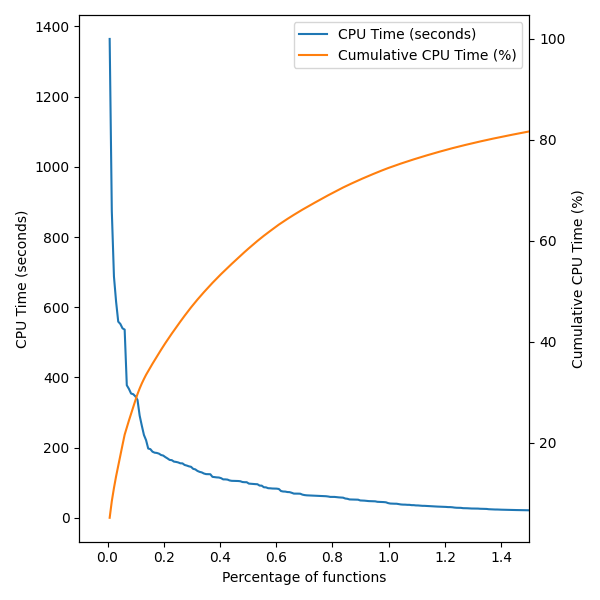
\includegraphics[width=\linewidth]{figures/global-longtail.png}
	\caption{Distribution of the functions' CPU time. The left y-axis shows the average total CPU Time spent in a function, while the right y-axis show the cumulative CPU time percentage. The x-axis percentage of functions ordered by decreasing CPU time. The data includes all functions from all pipelines.}
	\label{fig:long-tail-distribution}
\end{figure}
				
\subsection{Makespan: A performance overview}
Figure~\ref{fig:makespan-1thread} depicts the total time elapsed from the start to the end of each pipeline; i.e. makspan. There is a significant difference between the makespan of different applications. This is expected as the pipelines perform different tasks. The standard deviation is nearly null for all pipelines, except for FreeSurfer recon-all which as a small variation. Overall, this shows that the input data does not substantially affect the makespan of those pipelines.
			
\begin{figure}[t]
	\centering
	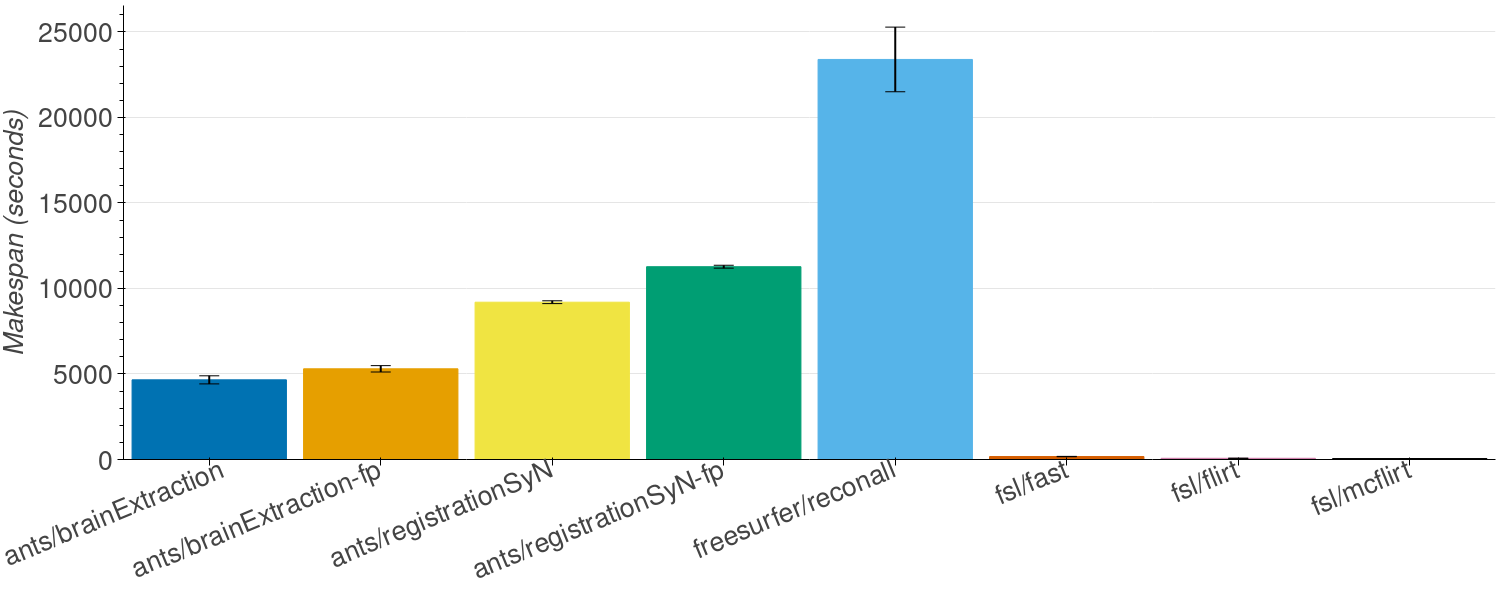
\includegraphics[width=\linewidth]{figures/makespan-1thread.png}
	\caption{Average makespan of the pipeline while using 1-thread. The error bars show the standard deviation. \TG{Font size in the figure is too small, it should be similar to the caption font size}}
	\label{fig:makespan-1thread}
\end{figure}
			
\subsection{Impact of Memory Bounded Functions}
Table~\ref{extab:memory-bound} shows that fetching data from disk is the main source of cycles where the CPU is starved. Following, The L1 bound has the highest cache-level contribution to the memory bound of the pipelines. ANTS pipelines have the highest L1 bound, followed by FreeSurfer recon-all and FSL MCFLIRT. L2 and L3 bound is low for all pipeline, although highest for FreeSurfer recon-all. The DRAM bound is high for both FSL FLIRT and FreeSurfer recon-all, followed by ANTS brainExtraction in single and double precision. Store bound is low for all pipelines. We note an interesting relationship between the low L1 bound and the high DRAM bound of FreeSurfer recon-all and FSL FLIRT, compared to the other pipelines.
			
\csvnames{csvcol}{1=\pipeline, 2=\mem, 3=\la, 4=\lb, 5=\lc, 6=\dram, 7=\store}
\csvstyle{memory_bound}{
	tabular = |r|c|c|c|c|c|c|,
	table head = \hline Pipeline &  \% Memory Bound &  \% L1 Bound &  \% L2 Bound &  \% L3 Bound & \% DRAM Bound & \% Store Bound\\\hline\hline,
	late after line = \\\hline,
	respect all,
	csvcol
}
\begin{table*}[ht]
	\centering
	\csvreader[memory_bound]{tables/memory_bound.csv}{}
	{\pipeline & \tablenum[round-precision=2]{\mem} & \tablenum[round-precision=2]{\la} & \tablenum[round-precision=2]{\lb} & \tablenum[round-precision=2]{\lc} & \tablenum[round-precision=2]{\dram} & \tablenum[round-precision=2]{\store}}
	\caption{Impact of data load on stalled CPU cycles. The values are the summation of the metric weighted by each function CPU time. This represent the percentage of the total CPU time stalled by each metrics. We show the average value across all subjects execution with one thread.}
	\label{extab:memory-bound}
\end{table*}
			
\subsection{Main Bottleneck: Linear Interpolation}
Table~\ref{extab:interpolation} shows that interpolation (or convolution) is a critical part for all pipelines, except FreeSurfer recon-all. For those pipelines, interpolation contributes between 32.20\% to 62.70\% of the total CPU time. Overall, the number of functions using interpolation is low with less than 20 in each applications. In other words, few interpolation functions are contribute to a large portion of the CPU time.
% There seems to be few  the stages from recon-all: https://surfer.nmr.mgh.harvard.edu/fswiki/recon-all (see section "Manual-Intervention Workflow Directives": stages 1-31)
			
\csvnames{csvcol}{1=\pipeline, 2=\nfunc, 3=\cputime}
\csvstyle{interpolation}{
	tabular = |r|c|c|,
	table head = \hline Pipeline & \# of functions & \% CPU Time \\
	& with interpolation & from interpolation\\\hline\hline,
	late after line = \\\hline,
	respect all,
	csvcol
}
\begin{table*}[h]
	\centering
	\csvreader[interpolation]{tables/interpolation.csv}{}
	{\pipeline & \nfunc & \tablenum[round-precision=2]{\cputime}}
	\caption{Contribution of interpolation to the applications' total CPU time. The percentage is the average sum of CPU time of functions using interpolation. The data includes all functions; not only the top 80\% of the CPU time.}
	\label{extab:interpolation}
\end{table*}
						
						
\subsection{ANTS: Single vs. Double Precision}
Figure~\ref{fig:makespan-ants} shows the makespan of ANTS brainExtraction and ANTS registrationSyN in double and single precision. For both pipelines, the makespan is significantly higher in single precision. This is unexpected, as the floating-point arithmetic operations are supposed to be faster in single precision~\cite{Wang2018-jv}.

\begin{figure}[h]
	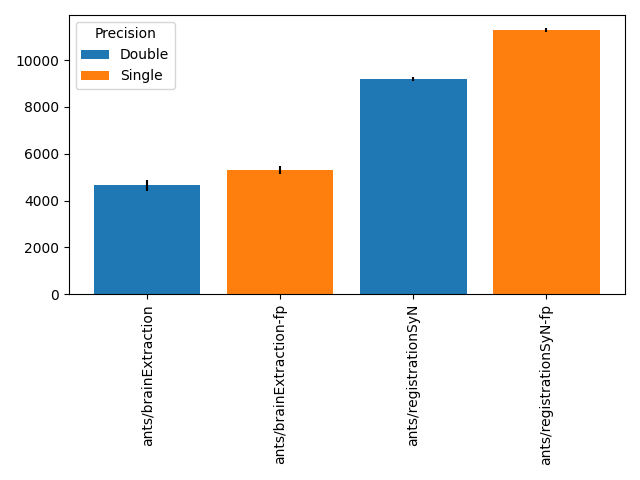
\includegraphics[width=\linewidth]{figures/makespan-ants.png}
	\caption{Comparison of makespan between double (blue) and single (orange) precision for ANTS brainExtraction and ANTS registrationSyN.}
	\label{fig:makespan-ants}
\end{figure}
			
The number of iteration between both version of ANTS registrationSyN is similar. In fact, for the latest two stages, they were the same across all but one execution. However, The single precision version of ANTS registrationSyN took longer per iteration than the double precision version (Figure~\ref{fig:mean-time-per-iteration-ants}). Therefore, the slowdown is not due to the convergence of the algorithm, but rather the execution time for each iteration.

\begin{figure}
	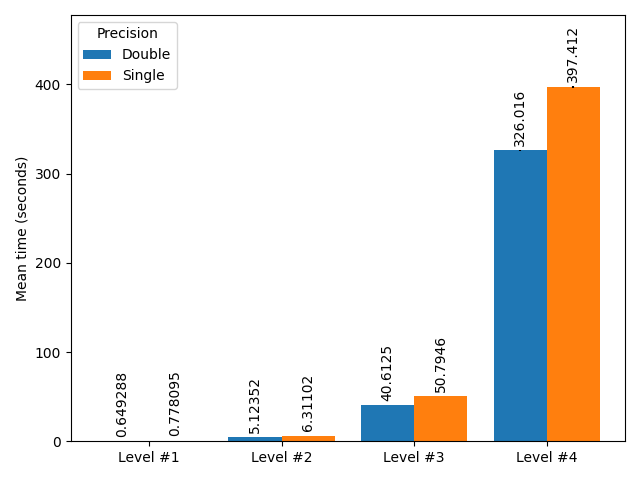
\includegraphics[width=\linewidth]{figures/ants-registrationSyN-iteration-mean.png}
	\caption{Mean time per iteration for ANTS registrationSyN in double and single precision. Only the SyN Registration stage is shown as the two earlier stage were near zero time. The error bars show the standard deviation.}
	\label{fig:mean-time-per-iteration-ants}
\end{figure}
						
\subsection{FreeSurfer: Thread-Synchronization}
Figure~\ref{fig:hotspots-freesurfer-reconall} shows a significant different in the pipeline profile between single-threaded and multi-threaded execution. The multi-threaded executions (Figure~\ref{subfig:hotspots-freesurfer-reconall-32threads}), OMP is a major bottleneck for the application, accounting for at least 76\% of the application runtime. FreeSurfer uses the multi-processing API provided by OpenMP. Moreover, the y-axis scale is multi folds larger than for the single-threaded executions. This indicates that the multi-threaded execution is significantly slower than the single-threaded execution.
					
\begin{figure*}
	\centering
	\begin{subfigure}[t]{0.49\textwidth}
		\caption{Single-threaded}
		\label{subfig:hotspots-freesurfer-reconall-1thread}
		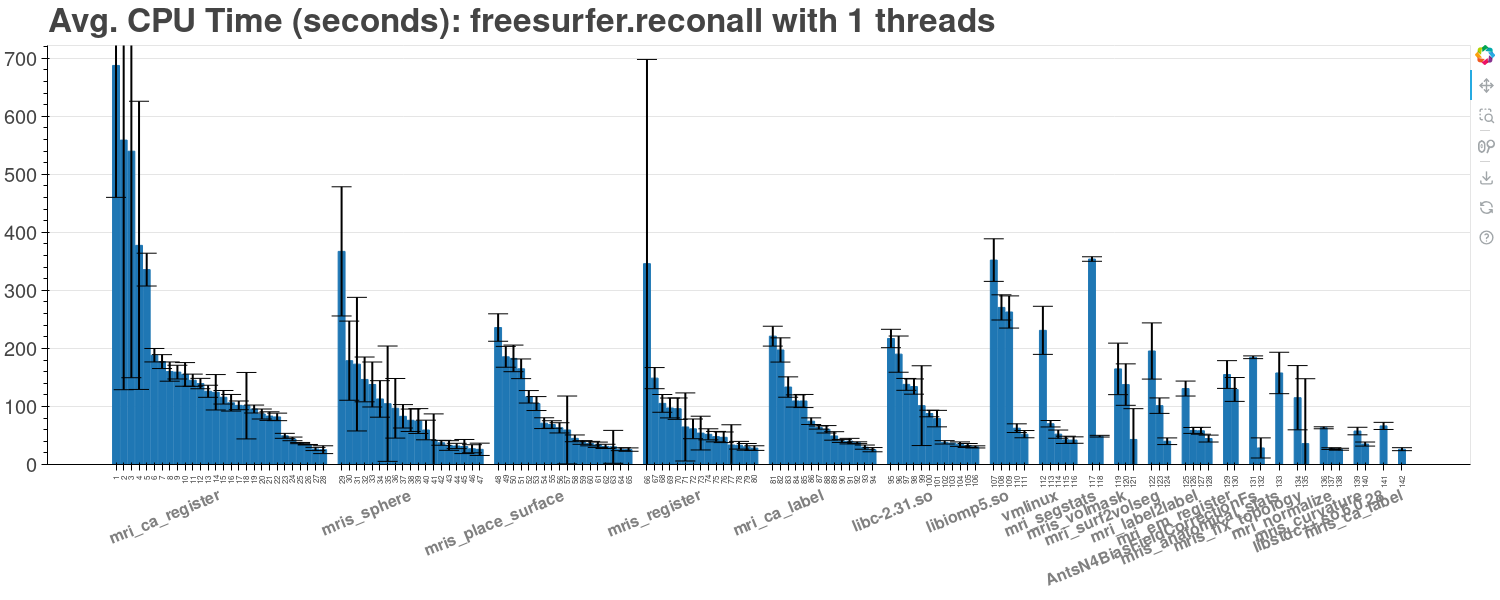
\includegraphics[width=\textwidth]{figures/hotspots-1threads-freesurfer-reconall-simple.png}
	\end{subfigure}
	\begin{subfigure}[t]{0.49\textwidth}
		\caption{Multi-threaded (32 threads)}
		\label{subfig:hotspots-freesurfer-reconall-32threads}
		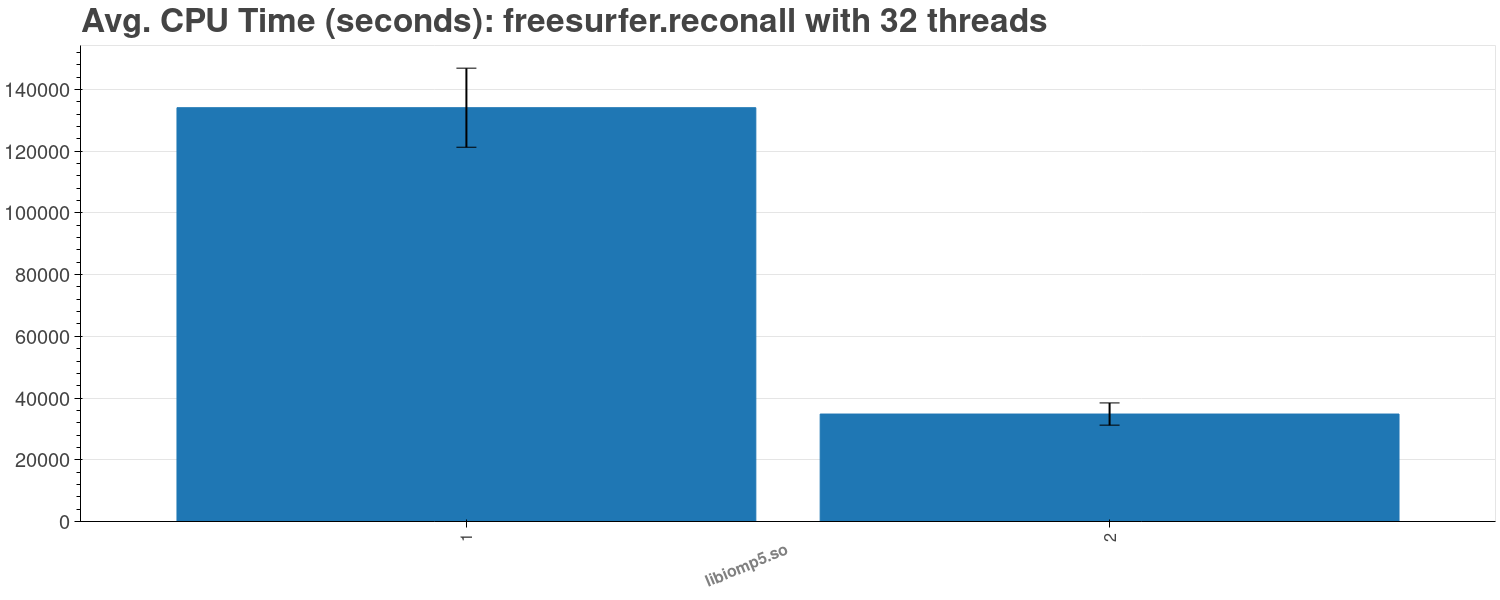
\includegraphics[width=\textwidth]{figures/hotspots-32threads-freesurfer-reconall-simple.png}
	\end{subfigure}
	\caption{FreeSurfer recon-all hotspots analysis. The y-axis show the average CPU time spent in each function, with error bars showing the standard deviation. The x-axis show the function ordered by decreasing CPU time grouped by module. We omit the function names for clarity. The function ID are dependent to each plot. The supplementary materials depicts the mapping of the function ID to the function name for each plot.}
	\label{fig:hotspots-freesurfer-reconall}
\end{figure*}
			
While the makespan for FreeSurfer recon-all decrease with an increase in the number of threads, the benefits are limited (Figure~\ref{fig:freesurfer-threading}). The parallel efficiency decreases from 66\% with two threads down to 5\% with 32 threads. While the Amdhals' law plays an impact on the maximum parallel efficiency of the pipeline, Figure~\ref{fig:hotspots-freesurfer-reconall} indicates that the thread Synchronization has a larger impact.
					
\begin{figure}
	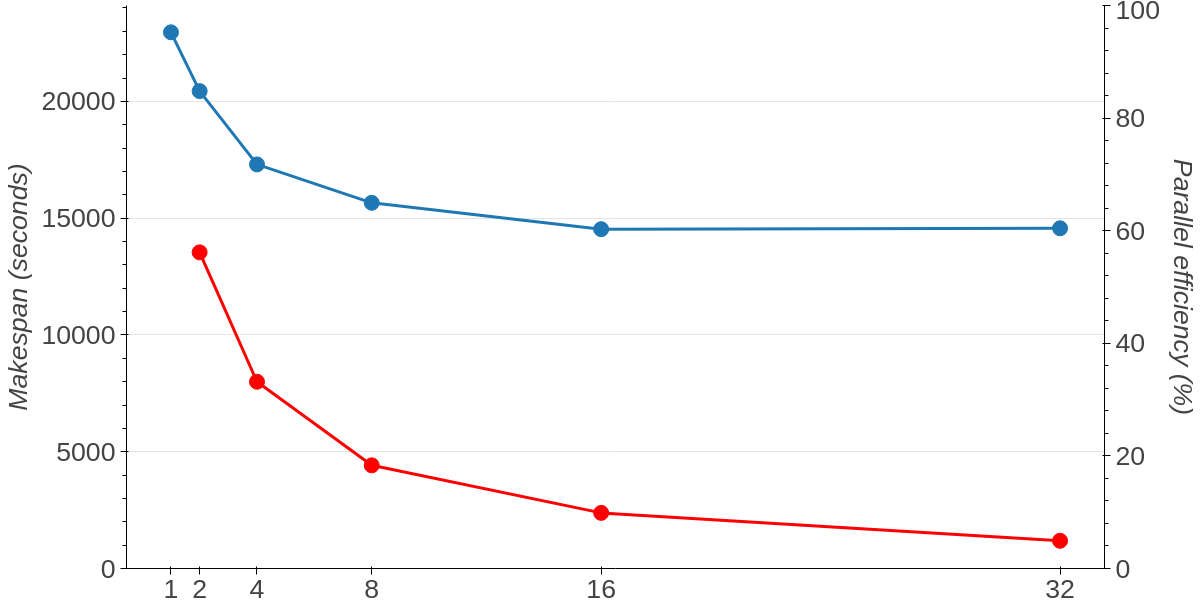
\includegraphics[width=\linewidth]{figures/makespan-freesurfer.png}
	\caption{Makespan and parallel efficiency of FreeSurfer recon-all while varying the number of threads between 1 to 32. The left y-axis shows the makespan in seconds, while the right y-axis shows the parallel efficiency in percent. The log-scaled x-axis shows the number of threads.}
	\label{fig:freesurfer-threading}
\end{figure}
								
\section{Discussion}
\subsection{Few functions account for most of the CPU time}
Our initial assumption was that the distribution of CPU time would follow a Pareto distribution. Thus, 20\% of the functions would contribute to 80\% of the total CPU time. However, Figure~\ref{fig:long-tail-distribution} shows that the distribution of CPU time is closer to a Zipf's law with exponent $\alpha=1.8$. This means that the CPU time of a function is approximately inversely proportional to its rank. This is consistent with the Pareto's principle, but is more extreme. Therefore, future efforts to optimize the main bottlenecks of MRI pre-processing pipelines could lead to enormous performance improvements.
			
\subsection{Wasted CPU cycles due to Memory Bound}
Overall, our results show a high percent of memory bound across all pipelines.
Optimizing the data access of the application could reduce the number of data load. This would potentially have a large impact on the performance of the pipelines. Alternatively, the use of reduced precision could reduce the memory footprint, thus the memory bound. To reduce the memory bound impact of fetching data from disk, it could be possible to convert and store the data to a lower precision before pre-processing. In both cases, the impact of reduced precision on the accuracy of the pipelines should be studied.
			
			
%%%%%%%%%% # Linear Interpolation
% Theoretical improvements using reduced precision. If time permits, toy experiment with ITK single precision data type at different locations.
% 1. Winograd algorithm for fast convolution.
% - It could be used to speed up the current pipeline. Tradeoff with precision? How does it compare to reduced precision?
% 2. Improvement to interpolation would help the current algorithms, as well as the DL algorithm using CNN.
\subsection{Importance of Linear Interpolation}
\MD{TODO}
			

%%%%%%%%%% # Single vs. Double Precision
% 1. Not as simple as using different data type. It could affect
% - Convergence
% - Accuracy
% - Runtime (maybe even slower)
% 1.5 Convergence is the sane in our case (same number of iterations).
% 2. Why is it slower in our case?
% -? Possibly less optimized code for single precision.
% -? Possibly memory placement
% -? ...
% 3. 
\subsection{ANTS: A tale of precision}
\MD{TODO + change title}


\subsection{OpenMP bottleneck in FreeSurfer recon-all}
In our experiments, FreeSurfer recon-all showed a significant decrease in parallel efficiency with an increase in the number of threads. While the Amdhals' law plays an impact on the maximum efficiency, the OpenMP thread synchronization played the largest impact in our results. The codebase use 83 \textit{static} scheduling policy out of 92 total. \textit{Static} scheduling assign chunks to threads in round-robin fashion. This could lead to a load imbalance between the threads, and thus a decrease in parallel efficiency. We supposed that \textit{dynamic} scheduling could improve the parallel efficiency, by assigning chunks based on the current load of the threads. Unfortunately, we failed to recompile FreeSurfer by naively changing the \textit{static} OpenMP scheduling to \textit{dynamic}. This remain challenging as the codebase is large and complex, and the change in scheduling policy could lead to unexpected bugs.
			
Future work should study the different configuration of OpenMP scheduling in FreeSurfer recon-all to improve the parallel efficiency. We believe that significant performance improvements could be achieved by optimizing the thread synchronization. This would lead to faster runtime time and higher CPU usage ration in HPC allocations.
			
\subsection{Limitations}
The dataset we chose contains wide range of age and equal distribution of sex. However, it only contains healthy subjects. Therefore, the performance bottleneck we found might not be applicable to data pre-processing of pathological patients. Moreover, the dataset is from a single site. This could also introduce bias from the scanner model and data acquisition protocol used. Future work should include data from multiple sites to ensure the generalization of the performance bottleneck we found.
			
Our analysis omits the space or time of execution for function calls. This information could provide additional insight for optimization. For example, spatial and temporal dimensions were shown to be important in the field of reduced precision. Future work could extent the depth of the analysis by including this information.
\MD{TODO Cite paper on spatial/temporal for RP (ask yohan for references)}
			
\section{Conclusion}
\MD{TODO}
			
			
\section{Data Availability}
\label{sec:data-availability}
The entire OpenNeuro ds004513 v1.0.2 dataset is freely available to download at:
\\\href{https://openneuro.org/datasets/ds004513/versions/1.0.2}{https://openneuro.org/datasets/ds004513/versions/1.0.2}.
	
The container images for our profiling experiments are publicly on Docker Hub:
\begin{itemize}
	\item mathdugre/cmake:debug-info
	\item mathdugre/intel-compilers:debug-info
	\item mathdugre/afni:debug-info
	\item mathdugre/ants:debug-info
	\item mathdugre/fsl:debug-info
	\item mathdugre/freesurfer:debug-info
	\item mathdugre/fmriprep:debug-info
\end{itemize}
	
Our profiling results from VTune are publicly available at:
\\\href{URL}{\MD{TODO add Zenodo link}}
	
\section{Code Availability}
\label{sec:code-availability}
The code to compile, profile the pipelines, and generate figures is publicly available at:
\\\href{https://github.com/mathdugre/mri-bottleneck}{https://github.com/mathdugre/mri-bottleneck}
\MD{TODO Update URL to slashbin org, when created.}
													
\section*{Acknowledgement}
\MD{TODO}
% NSERC PGS-D
% Concordia Bursary (find name)
% Any from others?
% ...
													
\section*{Conflict of Interests}
The authors report no conflict of interests.
													
\bibliographystyle{IEEEtran}
% \bibliography{IEEEabrv, paper}
\bibliography{paper}
													
\newpage
\onecolumn
\section*{Supplementary Materials}
\begin{figure*}
	\centering
	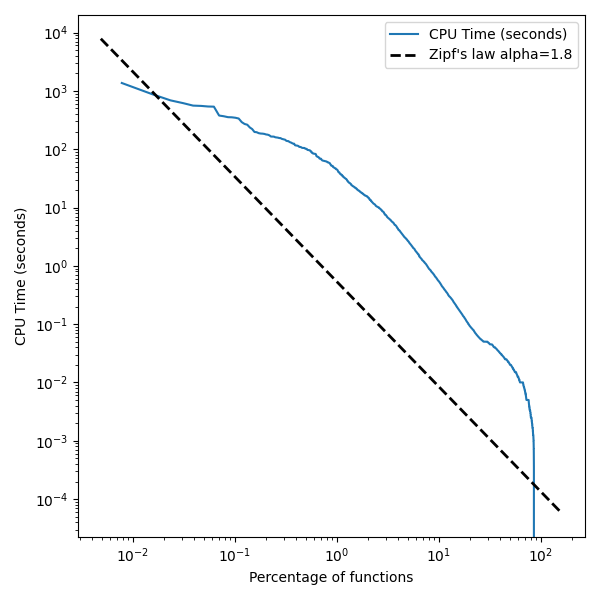
\includegraphics{figures/global-zipf_law.png}
	\caption{Distribution of the functions' CPU time compare to a Zipf's law distribution with $\alpha=1.8$. The y-axis shows the average CPU time for a function. The x-axis shows the percentage of functions ordered by decreasing CPU time. The data includes all functions from all pipelines.}
	\label{sup-fig:zips-law}
\end{figure*}
			
			
			
\label{sec:supplementary}
													
\csvnames{csvcol}{2=\module, 3=\func, 4=\mean, 5=\std}
\csvstyle{hotspot}{
	tabular = |r|l|l|c|,
	table head = \hline & Module & Function & CPU Time (mean$\pm$std)\\\hline\hline,
	late after line = \\\hline,
	respect all,
	csvcol
}
\newcommand{\csvtable}[3]{
	\begin{table}[h]
		\resizebox*{\textwidth}{!}{
			\csvreader[hotspot]{#1}{}
			% \csvreader[hotspot, filter={\value{csvrow}<60}]{#1}{}
			{\thecsvrow & \module & \func & \tablenum[round-precision=2, round-mode=places]{\mean}$\pm$\tablenum[round-precision=2, round-mode=places]{\std}}
		}
		\caption{#2}
		\label{#3}
	\end{table}
}
% CSV tables
% \csvtable{tables/hotspots-1thread-freesurfer-reconall.csv}{FreeSurfer recon-all (1 thread): Top functions accouting for 80\% of the application makespan.}{extab:hotspots-1thread-freesurfer-reconall}
\csvtable{tables/hotspots-32threads-freesurfer-reconall.csv}{FreeSurfer recon-all (32 threads): Top functions accouting for 80\% of the application makespan.}{extab:hotspots-32threads-freesurfer-reconall}
			
\end{document}
